\documentclass[tikz,border=2pt]{standalone}
\usepackage{amsmath}
\usepackage{amssymb}
\usepackage{xcolor}

\definecolor{journalink}{HTML}{1F1C18}
\definecolor{journalmuted}{HTML}{8A7F72}
\definecolor{journalaccent}{HTML}{9C2D2D}

\begin{document}
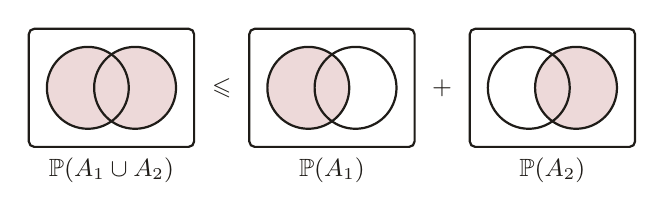
\begin{tikzpicture}[
  x=1cm,
  y=1cm,
  every node/.style={font=\small}
]
  \def\panelbox{(-0.75,-0.75) rectangle (1.35,0.75)}
  \def\circleA{(0,0) circle (0.52)}
  \def\circleB{(0.6,0) circle (0.52)}

  % Panel 1: P(A1 cup A2)
  \begin{scope}[shift={(0,0)}]
    \begin{scope}
      \clip \panelbox;
      \path[fill=journalaccent, fill opacity=0.18] \circleA;
      \path[fill=journalaccent, fill opacity=0.18] \circleB;
      \begin{scope}
        \clip \circleA;
        \path[fill=white] \circleB;
      \end{scope}
      \begin{scope}
        \clip \circleA;
        \path[fill=journalaccent, fill opacity=0.18] \circleB;
      \end{scope}
    \end{scope}
    \draw[journalink, line width=0.8pt, rounded corners=2pt] \panelbox;
    \draw[journalink, line width=0.8pt] \circleA;
    \draw[journalink, line width=0.8pt] \circleB;
    \node[journalink] at (0.3,-1.05) {$\mathbb{P}(A_1\cup A_2)$};
    \node[journalink] at (1.7,0) {$\leqslant$};
  \end{scope}

  % Panel 2: P(A1)
  \begin{scope}[shift={(2.8,0)}]
    \begin{scope}
      \clip \panelbox;
      \path[fill=journalaccent, fill opacity=0.18] \circleA;
    \end{scope}
    \draw[journalink, line width=0.8pt, rounded corners=2pt] \panelbox;
    \draw[journalink, line width=0.8pt] \circleA;
    \draw[journalink, line width=0.8pt] \circleB;
    \node[journalink] at (0.3,-1.05) {$\mathbb{P}(A_1)$};
    \node[journalink] at (1.7,0) {$+$};
  \end{scope}

  % Panel 3: P(A2)
  \begin{scope}[shift={(5.6,0)}]
    \begin{scope}
      \clip \panelbox;
      \path[fill=journalaccent, fill opacity=0.18] \circleB;
    \end{scope}
    \draw[journalink, line width=0.8pt, rounded corners=2pt] \panelbox;
    \draw[journalink, line width=0.8pt] \circleA;
    \draw[journalink, line width=0.8pt] \circleB;
    \node[journalink] at (0.3,-1.05) {$\mathbb{P}(A_2)$};
  \end{scope}
\end{tikzpicture}
\end{document}
